\documentclass[11pt,a4paper]{article}
% allow both latex and PDFlatex compatibility  (from pdfTeX FAQ)
\usepackage{hyperlatex}

\usepackage{pifont}
\usepackage{amsmath}
\usepackage{amssymb}
%\usepackage{psfig}
\usepackage{array}
\usepackage{supertabular}
%\usepackage{fancyheadings}
%\usepackage{here}
%\usepackage{pslatex}
\usepackage{eepic,epic}
%\usepackage{pslatex}%{\c c}a serait cens{\'e} corriger le pb de fontes dans les pdfs mais le fichier produit est pas beau
\usepackage[english]{babel}
\usepackage{alltt}

\texonly{\usepackage{graphicx}
\usepackage{makeidx}
\usepackage[pdftex,pageanchor=true,hyperindex=true,pagebackref=true,pdfhighlight=/O,pdfauthor={Yves Renard}]{hyperref}%pour le pdf
\usepackage{xspace} % insere un espace si necessaire 
\usepackage{underscore}
 %\usepackage{fancyheadings}
\usepackage{amsmath}
\usepackage{amssymb}
\usepackage{psfig}
\usepackage{here}
\usepackage{array}
\usepackage{alltt}
\usepackage{graphicx}
\usepackage{eepic,epic}
\usepackage[latin1]{inputenc}
\usepackage[T1]{fontenc}
% \usepackage[french]{babel}
% \usepackage[dvips]{epsfig}

%\oddsidemargin -0.2cm
%\evensidemargin -0.2cm
%\topmargin -1cm
%\textheight 22.5cm
%\textwidth 16.2cm
%\headheight 1.0cm

\newfont{\eufmtwelve}   {eufm10 scaled \magstep1}
\newfont{\eufmten}      {eufm10 }
\newfont{\eufmnine}     {eufm9 }
\newfont{\eufmeight}    {eufm8 }
\newfont{\eufmseven}    {eufm7 }
\newfont{\eufmsix}      {eufm6 }
\newfont{\eufmfive}     {eufm5 }
\newfont{\eusmtwelve}   {eusm10 scaled \magstep1}
\newfont{\eusmten}      {eusm10}
\newfont{\eusmnine}     {eusm9 }
\newfont{\eusmeight}    {eusm8 }
\newfont{\eusmseven}    {eusm7 }
\newfont{\eusmsix}      {eusm6 }
\newfont{\eusmfive}     {eusm5 }
\newfont{\msbmtwelve}   {msbm10 scaled \magstep1}
\newfont{\msbmeight}    {msbm8}

\newcommand{\udl}{\underline}
\newcommand{\udll}[1]{{\udl{\udl{#1}}}}
\newcommand{\udlll}[1]{{\udl{\udl{\udl{#1}}}}}
\newcommand{\mat}[1]{{\mbox{\msbmtwelve {#1}}}}
\newcommand{\Reel}{{\mbox{\msbmtwelve R}}}      % L'ensemble des reels.
\newcommand{\reel}{{\mbox{\msbmeight R}}}       % L'ensemble des reels.
%\newcommand{\Reel}{{\rm I\hspace{-0.15em}R}}
\newcommand{\Complex}{\mbox{\msbmtwelve C}}     % L'ensemble des complexes.
\newcommand{\Naturel}{\mbox{\msbmtwelve N}}  % L'ensemble des entiers naturels.
\newcommand{\naturel}{\mbox{\msbmeight N}}   % L'ensemble des entiers naturels.

%\newcommand{\Naturel}{{\rm I\hspace{-0.15em}N}}% L'ensemble des entiers naturels.
\renewcommand{\emptyset}{\mbox{$\circ$\hspace{-.50em}/}}  % ensemble vide.
\newcommand{\Cont}{{\cal C}}            % L'ensemble des fonctions continues
\newcommand{\Cinf}{{\cal C}^{\infty}}   % L'ensemble des fonction C-infinies
\renewcommand{\vec}[1]{\overrightarrow{\!\!#1}}
\newcommand{\subsetcont}{{\subset\hspace{-.6em}_{\scriptscriptstyle >} }}
\newcommand{\Frac}[2]{{\ds \frac{\ds #1}{\ds #2}}}
\newcommand{\interior}[1]{{\stackrel{\circ}{#1}}}
\newcommand{\cqfd}{{$\mbox{}$\hfill\rule{2.5mm}{2.5mm}}}
\newcommand{\vectwo}[2]{{\left(\hspace{-.5em}\begin{array}{c} {#1} \\ {#2}
     \end{array}\hspace{-.5em}\right)}}
\newcommand{\vecthree}[3]{{\left(\hspace{-.5em}\begin{array}{c} {#1}
     \\ {#2} \\ {#3} \end{array}\hspace{-.5em}\right)}}
\newcommand{\vecfour}[4]{{\left(\hspace{-.5em}\begin{array}{c} {#1}
     \\ {#2} \\ {#3} \\ {#4} \end{array}\hspace{-.5em}\right)}}
\newcommand{\vecfive}[5]{{\left(\hspace{-.5em}\begin{array}{c} {#1}
     \\ {#2} \\ {#3} \\ {#4} \\ {#5} \end{array}\hspace{-.5em}\right)}}
\newcommand{\vecseven}[7]{{\left(\hspace{-.5em}\begin{array}{c} {#1}
     \\ {#2} \\ {#3} \\ {#4} \\ {#5} \\ {#6} \\ {#7} \end{array}\hspace{-.5em}\right)}}
\def\infess{\mathop{\iflanguage{english}{\mbox{ess$\,$inf}}{\mbox{inf$\,$ess}}}}
\def\supess{\mathop{\iflanguage{english}{\mbox{ess$\,$sup}}{\mbox{sup$\,$ess}}}}
\def\essinf{\mathop{\iflanguage{english}{\mbox{ess$\,$inf}}{\mbox{inf$\,$ess}}}}
\def\esssup{\mathop{\iflanguage{english}{\mbox{ess$\,$sup}}{\mbox{sup$\,$ess}}}}
\def\aplim{\mathop{\mbox{ap$\,$lim}}}
\def\aplimsup{\mathop{\mbox{ap$\,$lim$\,$sup}}}
\def\apliminf{\mathop{\mbox{ap$\,$lim$\,$inf}}}
\def\convto{\mathop{\hbox{\rightarrowfill}}} % converge vers.
\newcommand{\rightgap}{{]\hspace{-0.12em}]}}
\newcommand{\leftgap}{{[\hspace{-0.12em}[}}
\newcommand{\gapof}[1]{{\leftgap {#1} \rightgap}}
\newcommand{\restrictiona}[1]
{{ \begin{picture}(13,10) \put(-1,-4){$\mid_{#1}$} \end{picture}
}} % Le signe "Restriction sur #1"

\def\Indic{\mbox{1\hspace{-0.20em}I}}   % Fonction l'indicatrice

% \def\bar3{|\hspace{-1pt}\|} % 3bar verticaux pour les normes matricielles.
\def\cvweak{\mathop{-\hspace{-0.3em}-\hspace{-0.6em}\rightharpoonup}} % fleche cv faible
\def\cvweakstar{\cvweak^*} % fleche cv faible etoile
\def\longmapsto
{ \begin{picture}(0,10)
  \put(0,0){$\scriptstyle{\vdash}$} \end{picture} \mbox{$\longrightarrow$}
} 

\def\build#1_#2^#3{\mathrel{
 \mathop{\kern 0pt#1}\limits_{#2}^{#3}}} % Ecrire en dessous et dessus un symbole.

\def\Dist{\mbox{\eusmtwelve D}} %signe de distribution
\def\dist{\mbox{\eusmten D}} %signe de distribution


%definition de commandes utilises
\newcommand{\ds}{\displaystyle}
\newcommand{\rc}{{\par}}
\newcommand{\rcc}{{\par\medskip}}
\newcommand{\rccc}{{\par\bigskip}}


%definition des environnements theoreme, lemme, ...
\usepackage{boxedminipage}
% \newenvironment{largebox}
%   { \rc\noindent \begin{boxedminipage}[t]{\textwidth} }
%   { \end{boxedminipage}  \rccc\noindent }
\newenvironment{largebox}
  { \rc\noindent \begin{boxedminipage}[t]{\linewidth} }
  { \end{boxedminipage}  \rccc\noindent }


\newtheorem{ltheoreme}{Th\'eor\`eme}
\newenvironment{theoreme}
  { \begin{largebox} \begin{ltheoreme} }
  { \end{ltheoreme} \end{largebox} }
\newtheorem{lproposition}{Proposition}
\newenvironment{proposition}
  { \begin{largebox} \begin{lproposition} }
  { \end{lproposition} \end{largebox} }
\newtheorem{llemme}{Lemme}
\newenvironment{lemme}
  { \begin{largebox} \begin{llemme} }
  { \end{llemme} \end{largebox} }
\newtheorem{ldefinition}{D\'efinition}
\newenvironment{definition}
  { \begin{largebox} \begin{ldefinition} }
  { \end{ldefinition} \end{largebox} }
\newtheorem{lhypothese}{Hypoth\`ese}
\newenvironment{hypothese}
  { \begin{largebox} \begin{lhypothese} }
  { \end{lhypothese} \end{largebox} }
\newtheorem{lcorollaire}{Corollaire}
\newenvironment{corollaire}
  { \begin{largebox} \begin{lcorollaire} }
  { \end{lcorollaire} \end{largebox} }
\newenvironment{remarque}
  { \begin{largebox} {\bf \udl{Remarque} : }}
  { \end{largebox} }

\newcounter{numberofprobl}
\setcounter{numberofprobl}{1}

\newlength{\compteurtpourprobla}
\newlength{\compteurtpourproblb}
\newenvironment{caseeqnarray}[1]
  {
   $${#1}
   \settowidth{\compteurtpourprobla}{${#1}\left\{\right.$}
   \setlength{\compteurtpourproblb}{\textwidth}
   \addtolength{\compteurtpourproblb}{-1\compteurtpourprobla}
   \settowidth{\compteurtpourprobla}{$\;$}
   \addtolength{\compteurtpourproblb}{-1\compteurtpourprobla}
   \left\{ \begin{minipage}[l]{\compteurtpourproblb}
   \vspace{-1em} \begin{eqnarray}
  }
  { \end{eqnarray} \end{minipage} \right. $$}


\newtheorem{hypothesis}{Hypothesis}
\newtheorem{prop}{Proposition}
\newtheorem{defi}{Definition}
%\newtheorem{theorem}{Theorem}
%\newtheorem{lemma}{Lemma}


% pour plus tard ...
% \DeclareGraphicsRule{ps.Z}{eps}{ps.bb}{`zcat #1}
% \DeclareGraphicsRule{eps.Z}{eps}{eps.bb}{`zcat #1}
% \DeclareGraphicsRule{ps.gz}{eps}{ps.bb}{`gunzip #1}
% \DeclareGraphicsRule{eps.gz}{eps}{eps.bb}{`gunzip #1}

\newcommand{\ds}{\displaystyle}
\newcommand{\Frac}[2]{{\ds \frac{\ds #1}{\ds #2}}}
\oddsidemargin -0.9cm
\evensidemargin -0.9cm
\topmargin -1cm
\textheight 22.5cm
\textwidth 17.6cm
\headheight 1.0cm
}
\makeindex

% \W .. is equivalent to \htmlonly{..}
\W \newcommand{\HlxIcons}{./}
\W \usepackage{frames} % navigation panel
\W \htmldirectory{getfemuser}
\W \htmlname{getfemuser}
\W \setcounter{htmldepth}{2}
\W \setcounter{htmlautomenu}{2}
\W \renewcommand{\HlxMeta}{\xml{META description="getfem++ user manual"}}
\htmlonly{
  \htmlpanelfield{Index}{getfemuser}
  \htmlcss{getfemuser.css}
  \newcommand{\text}[1]{\mathrm{#1}}
  \newcommand{\WEB}[2]{\xmlattributes*{a}{target="_top"}\xlink{#2}{#1}}
  \newcommand{\nabla}{\htmlsym{nabla}}%renamed \xmlent by lastest version of hyperlatex
  \newcommand{\ell}{\htmlsym{tau}}
  \newcommand{\lambda}{\htmlsym{lambda}}
  \newcommand{\varepsilon}{\htmlsym{epsilon}}
  \newcommand{\phi}{\htmlsym{phi}}
  \newcommand{\varphi}{\htmlsym{phi}}
  \newcommand{\psi}{\htmlsym{psi}}
  \newcommand{\sigma}{\htmlsym{sigma}}
  \newcommand{\nu}{\htmlsym{nu}}
  \newcommand{\beta}{\htmlsym{beta}}
  \newcommand{\gamma}{\htmlsym{gamma}}
  \newcommand{\Gamma}{\htmlsym{Gamma}}
  \newcommand{\Delta}{\htmlsym{Delta}}
  \newcommand{\delta}{\htmlsym{delta}}
  \newcommand{\Omega}{\htmlsym{Omega}}
  \newcommand{\omega}{\htmlsym{omega}}
  \newcommand{\partial}{\htmlsym{part}}
  \newcommand{\sum}{\htmlsym{sum}}
  \newcommand{\int}{{\Large\htmlsym{int}}}
}
\T \newcommand{\Div}{\textrm{div}}
\W \newcommand{\Div}{div}
\T \newcommand{\Grad}{\textrm{grad}}
\W \newcommand{\Grad}{grad}
\T \newcommand{\Rot}{\textrm{curl}}
\W \newcommand{\Rot}{curl}

\W \newcommand{\gf}{getfem++}
\T \newcommand{\gf}{{\sc Getfem++}\xspace}

\W \newcommand{\newpage}{}
\W \newcommand{\hspace}[1]{ }
\W \newcommand{\left}{} % pour les left\(i\right) 
\W \newcommand{\right}{}
\W \newenvironment{alltt}{\begin{example}}{\end{example}}
\T \newenvironment{cppcode}{\begin{alltt}}{\end{alltt}}
\W \newenvironment{cppcode}{\begin{rawxml}<div class="cppcode">\end{rawxml}\begin{example}}{\end{example}\begin{rawxml}</div>\end{rawxml}}
\T \newcommand{\cpp}[1]{\texttt{#1}}
\T \newcommand{\filename}[1]{\texttt{#1}}
\W \newcommand{\cpp}[1]{\xmlattributes*{tt}{class="inlinecppcode"}\texttt{#1}}
\W \newcommand{\filename}[1]{\xmlattributes*{tt}{style="color:red"}\texttt{#1}}

\T \newenvironment{ctableau}[2]{\begin{center}\begin{supertabular}{#1}}{\end{supertabular}\end{center}}
\W \newenvironment{ctableau}[2]{\xmlattributes*{table}{border=1 align="center"}\begin{tabular}{#2}}{\end{tabular}}
\begin{document}

\begin{center}
\texonly{
  
\includegraphics[width=10cm,angle=0]{getfemlogo}\\[0.2cm]
  a Generic Finite Element library in C++ \\[0.5cm]
  {\LARGE Documentation, part \Huge 2} \\[0.5cm]
  \fbox{\Huge \sc Short User Documentation} \\[0.5cm]
  { \large Yves {\sc Renard}, Julien {\sc Pommier} \footnote{ \it MIP, INSAT, Complexe scientifique de Rangueil, 31077 Toulouse, France, Yves.Renard@gmm.insa-tlse.fr } } \\[1.0cm]
  \today \\[1.0cm]
}
\htmlonly{
  \xmlattributes*{a}{target="_top"}\xlink{\htmlimg{getfemlogo.png}{the getfem logo}}{http://www.gmm.insa-tlse.fr/getfem}\\[2cm]
  a Generic Finite Element library in C++ \par\par
  {\LARGE Documentation, part \Huge 2} \par\par
  {\Huge Short User Documentation } \par
  { \large \xlink{Yves Renard}{mailto:Yves.Renard@gmm.insa-tlse.fr}, \xlink{Julien Pommier}{mailto:Julien.Pommier@gmm.insa-tlse.fr}}\\
  {\it MIP, INSAT, Complexe scientifique de Rangueil, 31077 Toulouse, France.}\par
  \today \par\par
}
\end{center}

% \begin{abstract}
% Basic user documentation for \gf .
% \end{abstract}


%%%%%%%%%%%%%%%%%%%%%%%%%%%%%%%%%%%%%%%%%%%%%%%%%%%%%%%%%%%%%%%%%%%%%%%%%
%          INTRODUCTION                                                 %
%%%%%%%%%%%%%%%%%%%%%%%%%%%%%%%%%%%%%%%%%%%%%%%%%%%%%%%%%%%%%%%%%%%%%%%%%

\section*{Introduction}

The \gf project is centered around the development of a generic and efficient elementary computations C++ library for finite element methods. The goal is to build a library which allows to compute any elementary matrix (even for mixed methods) on the largest class of methods and elements and for arbitrary dimension. It offers a complete separation between integration methods (exact or approximated), geometric transformations (linear or not) and finite element methods of arbitrary degrees. It allows to write finite element code which are independent of the particular method, and thus to test easily various finite element method on the same problem.

 Moreover, the library includes other tools for computation with finite element such as assembling methods for classical PDEs, interpolation methods, computation of norms, mesh operations, boundary conditions ... This library allows to build finite elements codes which are completely independent of the dimension, the particular method or element. Examples are provided.\\[2cm]
\htmlonly{\\\\\\}
Copyright (C) 2000-2020 Yves Renard, Julien Pommier.\\
The program GetFEM is free software; you can redistribute it and/or modify
it under the terms of the GNU Lesser General Public License as published by
the Free Software Foundation; either version 3 of the License, or
(at your option) any later version along with the GCC Runtime Library
Exception either version 3.1 or (at your option) any later version.
This program is distributed in the hope that it will be useful,
but WITHOUT ANY WARRANTY; without even the implied warranty of
MERCHANTABILITY or FITNESS FOR A PARTICULAR PURPOSE.  See the
GNU Lesser General Public License for more details.
You should have received a copy of the GNU  Lesser General Public License
along with this program; if not, write to the Free Software Foundation,
Inc., 51 Franklin Street, Fifth Floor, Boston, MA  02110-1301  USA

\newpage
\tableofcontents
\newpage

\section{How to install}
\index{Install}
Since we used standard GNU tools, the installation of the \gf  library is somewhat standard. If the \gf  archive is on your current directory you can unpack it and enter inside the directory of the distribution  with the commands
\begin{alltt}
  gunzip -c getfem-x.xx.tar.gz | tar xvf -
  cd  getfem-x.xx
\end{alltt}
Then you you have to run the configure script just typing
\begin{alltt}
  ./configure
\end{alltt}
or if you want to set the prefix directory where to install the library you can use the {\tt {-}{-}prefix} option (the default prefix directory is {\tt /usr/local}):
\begin{alltt}
  ./configure --prefix=\textit{dest_dir}
\end{alltt}
then start the compilation with
\begin{alltt}
  make
\end{alltt}
(or preferably with {\tt gmake}) and the installation with
\begin{alltt}
  make install
\end{alltt}
You can also check if the compilation is correct with
\begin{alltt}
  make check
\end{alltt}

If you want to use a different compiler than the one chosen
automatically by the \texttt{./configure} script, just specify its
name on the command line:
\begin{alltt}
  ./configure CXX=mycompiler
\end{alltt}
More specific instructions can be found in the \texttt{README*} files of
the distribution.

\section{Build a mesh}
\index{mesh}
\gf  has it own structure to store meshes defined in the files \filename{bgeot\_mesh\_structure.h}, \filename{bgeot\_mesh.h} and \filename{getfem\_mesh.h}. The main structure is defined in \filename{getfem\_mesh.h} by the object\\[0.5cm]
\cpp{getfem::getfem\_mesh }\\[0.5cm]
This object is able to store any element in any dimension even if you mix elements with different dimensions.\\[0.5cm]

There is no meshing procedures in \gf  to mesh complex geometries. This is not the goal of this package. But you can easily load a mesh from any format (some procedures are in \filename{getfem_import.h} to load meshes from some public domain mesh generator).

\subsection{Add an element to a mesh}
Suppose the variable mesh has been declared by
\index{GETFEM!getfem::getfem_mesh}
\begin{cppcode}
  getfem::getfem\_mesh mesh;
\end{cppcode}
then you have two ways to insert a new element to this mesh : from a list of points or from a list of indexes of already existing points.\\[0.5cm]
To enter a new point on a mesh use the method\\[0.5cm]
\index{GETFEM!mesh.add_point(pt)}
\cpp{i = mesh.add\_point(pt);}\\[0.5cm]
where \cpp{pt} is of type \cpp{bgeot::base\_node}. The index \cpp{i} is the index of this point on the mesh. If the point already exists in the mesh, a new point is not inserted and the index of the already existing point is returned. A mesh has a principal dimension, which is the dimension of its points. It is not possible to have points of different dimensions in a same mesh.\\[0.5cm]
The more basic function to add a new element to a mesh is\\[0.5cm]
\index{GETFEM!mesh.add_convex(pgt, it)}
\cpp{j = mesh.add\_convex(pgt, it);}\\[0.5cm]
This is a template function, with \cpp{pgt} of type \cpp{bgeot::pgeometric\_trans} and \cpp{it} is an iterator on a list of indexes of already existing points. For instance, if one needs to add a new triangle in a 3D mesh, one needs to define first an array with the indexes of the three points:\\[0.5cm]
\begin{cppcode}
  std::vector<bgeot::size\_type> ind(3);
  ind[0] = mesh.add\_point(bgeot::base\_node(0.0, 0.0, 0.0);
  ind[1] = mesh.add\_point(bgeot::base\_node(0.0, 1.0, 0.0);
  ind[2] = mesh.add\_point(bgeot::base\_node(0.0, 0.0, 1.0);
\end{cppcode}
then adding the element is done by\\[0.5cm]
\cpp{mesh.add\_convex(bgeot::simplex\_trans(2,1), ind.begin()); }\\[0.5cm]
\index{BGEOT!bgeot::simplex\_trans(N,1)}
where \cpp{bgeot::simplex\_trans(N,1);} denotes the usual linear geometric transformation for simplexes of dimension N.\\[0.5cm]
For simplexes, a more specialized function exists, which is\\[0.5cm]
\cpp{mesh.add\_simplex(2, ind.begin()); }\\[0.5cm]

It is also possible to give directly the list of points with the function\\[0.5cm]
\index{GETFEM!mesh.add\_convex\_by\_points(pgt, itp)}
\cpp{mesh.add\_convex\_by\_points(pgt, itp); }\\[0.5cm]
where now \cpp{itp} is an iterator on an array of points. For example\\[0.5cm]
\begin{cppcode}
  std::vector<bgeot::base\_node> pts(3);
  pts[0] = bgeot::base\_node(0.0, 0.0, 0.0);
  pts[0] = bgeot::base\_node(0.0, 1.0, 0.0);
  pts[0] = bgeot::base\_node(0.0, 0.0, 1.0);
  mesh.add\_convex\_by\_points(bgeot::simplex\_trans(2,1), pts.begin());
\end{cppcode}
Still add a triangle to the mesh.
It is possible to use also \\[0.5cm]
\cpp{mesh.add\_simplex\_by\_points(2, pts.begin()); } \\[0.5cm]

For other elements than simplexes, it is still possible to use \cpp{mesh.add\_convex\_by\_points} or $\ $$\ $ \cpp{mesh.add\_convex} with the appropriate geometric transformation. \\[0.5cm]
\index{BGEOT!bgeot::parallelepiped\_trans(N, 1)}
\cpp{bgeot::parallelepiped\_trans(N, 1) }
describes the usual transformation for parallelepipeds of dimension \cpp{N} (quadrilateron for \cpp{N=2}, hexahedron for \cpp{N=3}, ...) \\[0.5cm]
\index{BGEOT!bgeot::prism\_trans(N, 1)}
\cpp{bgeot::prism\_trans(N, 1) } 
describes the usual transformation for prisms of dimension \cpp{N} (usual prism is for \cpp{N=3}. A generalized prism is the product of a simplex of dimension \cpp{N-1} with a segment) \\[0.5cm]
Specialized functions exist also: \\[0.5cm]
\begin{cppcode}
  mesh.add\_parallelepiped(N, it);
  mesh.add\_parallelepiped\_by\_points(N, itp);
  mesh.add\_prism(N, it);
  mesh.add\_prism\_by\_points(N, itp);
\end{cppcode}

The order of the points in the array of point is not important for simplexes. For other element, it is important to respect the order shown in figure \ref{fig:elem}.

\begin{figure}[htb]
  \begin{center}
    \texonly{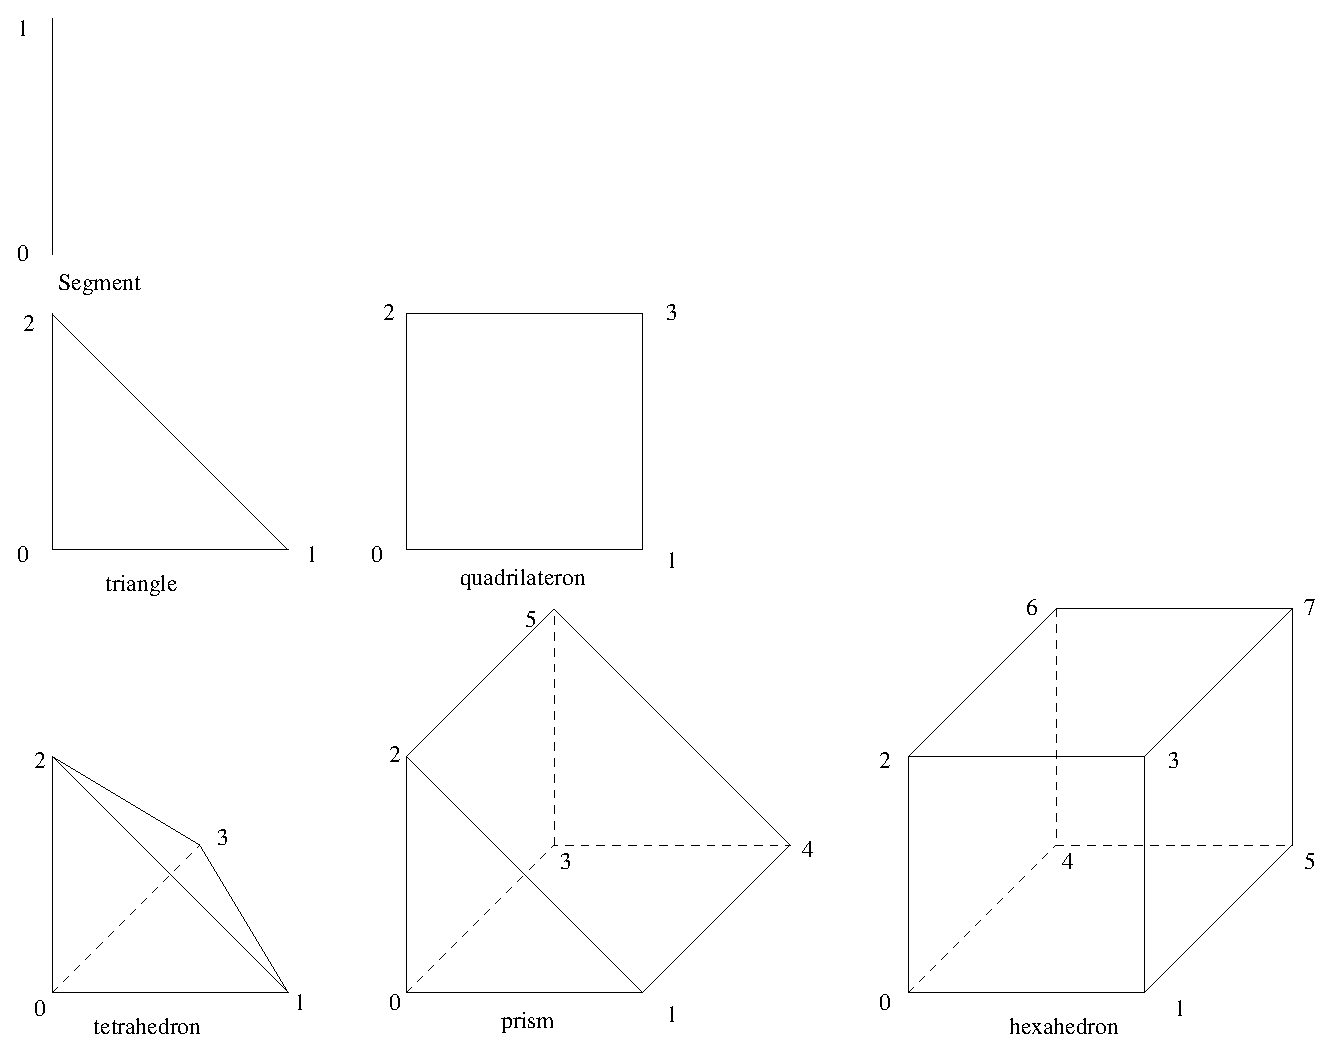
\includegraphics[width=15cm,angle=0]{getfemuserelem}}
    \htmlonly{\htmlimg{getfemuserelem.png}{vertex numeration for usual elements}}
  \end{center}
  \caption{ \it vertex numeration for usual elements }
  \label{fig:elem}
\end{figure}

\subsection{Remove an element from a mesh}
To remove an element from a mesh, simply use\\[0.5cm]
\index{GETFEM!mesh.sup\_convex(i)}
\cpp{mesh.sup\_convex(i); }\\[0.5cm]
where \cpp{i} is the index of the element.

\subsection{Simple structured meshes}

For parallelepiped domains, it is possible to obtain structured meshes with simplexes, parallelepipeds or prisms elements from three functions defined in \cpp{getfem\_regular\_meshes.h}. \\[0.5cm]
\index{GETFEM!getfem::parallelepiped\_regular\_mesh}
\begin{cppcode}
  getfem::parallelepiped\_regular\_simplex\_mesh(mesh, N, org, ivect, iref); \\
  getfem::parallelepiped\_regular\_prism\_mesh(mesh, N, org, ivect, iref); \\
  getfem::parallelepiped\_regular\_mesh(mesh, N, org, ivect, iref);
\end{cppcode}
where \cpp{mesh} is a mesh variable in which the structured mesh will be built, \cpp{N} is the dimension (limited to 4 for simplexes, 5 for prisms, unlimited for parallelepipeds), \cpp{org} is of type \cpp{bgeot::base\_node} and represents the origin of the mesh, \cpp{ivect} is an iterator on an array of \cpp{N} vectors to build the parallelepiped domain, \cpp{iref} is an iterator on an array of \cpp{N} integers representing the number of division on each direction. \\[0.5cm]
For instance, to build a mesh with tetrahedrons for a unit cube with $10\times10\times10$ cells one can write\\[0.5cm]
\begin{cppcode}
  getfem::getfem\_mesh mesh; \\
  bgeot::base\_node org(0.0, 0.0, 0.0); \\
  std::vector<bgeot::base\_vector> vect(3); \\
  vect[0] = bgeot::base\_vector(1.0, 0.0, 0.0); \\
  vect[1] = bgeot::base\_vector(0.0, 1.0, 0.0); \\
  vect[2] = bgeot::base\_vector(0.0, 0.0, 1.0); \\
  std::vector<int> ref(3); \\
  ref[0] = ref[1] = ref[2] = 10; \\
  getfem::parallelepiped\_regular\_simplex\_mesh(mesh, 3, org, vect.begin(), ref.begin()); 
\end{cppcode}


\subsection{How to get information from a mesh}

Here is a list of functions to get information from an existing mesh. The list is not exhaustive.

\begin{ctableau}{|m{0.4\linewidth}|m{0.55\linewidth}|}{ll}\hline
  \cpp{mesh.dim()} & main dimension of the mesh.  \\ \hline

  \cpp{mesh.points\_index()} & gives a \cpp{dal::bit\_vector} object which represents all the indexes of valid points of a mesh (see in the following)  \\ \hline

  \cpp{mesh.points()[i]} & gives the point of index \cpp{i} (a \cpp{bgeot::base\_node} ). \\ \hline
  
  \cpp{mesh.convex\_index()} & gives a \cpp{dal::bit\_vector} object which represents all the indexes of valid elements of a mesh (see in the following) \\ \hline

  \cpp{mesh.structure\_of\_convex(i)} & gives the description of the structure of element of index \cpp{i}. The function return a \cpp{bgeot::pconvex\_structure}. \\ \hline

  \cpp{mesh.structure\_of\_convex(i)\hspace{5em}->nb_faces()} & number of faces of  element of index \cpp{i}. \\ \hline

  \cpp{mesh.structure\_of\_convex(i)\hspace{5em}->nb\_points()} & number of vertices of  element of index \cpp{i}. \\ \hline

  \cpp{mesh.structure\_of\_convex(i)->dim()} & intrinsic dimension of element of index \cpp{i}. \\ \hline

  \cpp{mesh.structure\_of\_convex(i)\hspace{5em}->nb\_points\_of\_face(f)} & number of vertices of the face of local index \cpp{f} of  element of index \cpp{i}.\\ \hline
 
  \cpp{mesh.structure\_of\_convex(i)\hspace{5em}->ind\_points\_of\_face(f)} & return a container with the local indexes of all vertices of the face of local index \cpp{f} of  element of index \cpp{i}. For instance \cpp{mesh.structure\_of\_convex(i) ->ind\_points\_of\_face(f)[0]} is the local index of the first vertex. \\ \hline

  \cpp{mesh.structure\_of\_convex(i)\hspace{5em}->face\_structure(f)} & gives the structure (a \cpp{bgeot::pconvex\_structure}) of local index \cpp{f} of  element of index \cpp{i}.\\ \hline

  \cpp{mesh.ind\_points\_of\_convex(i)} & gives a container with the global indexes of  vertices of element of index \cpp{i}.\\ \hline

  \cpp{mesh.points\_of\_convex(i)} & gives a container with the  vertices of element of index \cpp{i}. This is an array of \cpp{bgeot::base\_node}.\\ \hline

  \cpp{mesh.convex\_to\_point(ipt)} & gives a container with the indexes of all elements attached to the point of global index \cpp{ipt}.\\ \hline

  \cpp{convex\_with\_points(mesh, nb, ipts) } & gives a container with the indexes of all elements in \cpp{mesh} having a certain set of points for vertices. The set of points is describe by an iterator \cpp{ipts} on an array and the number of points \cpp{nb}.\\ \hline

  \cpp{neighbour\_of\_convex(mesh, ic, f)} & gives a container with the indexes of all elements in \cpp{mesh} having the common face of local index \cpp{f} of element \cpp{ic} except element \cpp{ic}. \\ \hline

  \cpp{mesh.stat()} & print in \cpp{std::cout} main information on the mesh. \\ \hline

  \cpp{mesh.clear()} & delete all elements and points from the mesh. \\ \hline

  \cpp{mesh.optimize\_structure()} & compact the structure. \\ \hline

  \cpp{mesh.trans\_of\_convex(i)} & geometric transformation of the element of index \cpp{i}. return a \cpp{bgeot::pgeometric\_trans} (see \cite{BASCOMP} for more details).  \\ \hline

  \cpp{mesh.normal\_of\_face\_of\_convex(ic, f, pt)} & gives a \cpp{bgeot::base\_vector} representing an outward normal to the element at the face of local index \cpp{f} at the point of local coordinates (coordinates in the element of reference) \cpp{pt}. The point \cpp{pt} has no influence if the geometric transformation is linear. This is not a unit normal, the norm of the resulting vector is the ratio between the surface of the face of the reference element and the the surface of the face of the real element. \\ \hline

\end{ctableau}

\index{DAL!dal::bit\_vector}
About the object \cpp{dal::bit\_vector}, which is very close to \cpp{std::bit\_vector} but with additional functionalities to represent a set of non negative integers. If \cpp{nn} is declared to be a \cpp{dal::bit\_vector}, the two instructions \cpp{nn.add(6)} or \cpp{nn[6] = true} are equivalent and means that integer 6 is added to the set. In a same way \cpp{nn.sup(6)} or \cpp{nn[6] = false} remove the integer 6 from the set. The instruction \cpp{nn.add(6, 10)} add the whole interval from 6 to 10 to the set (i.e. here 6, 7, 8, 9 and 10). To iterate on a \cpp{dal::bit\_vector}, it is possible to use iterators as usual,  but, most of the time, as this object represents a set of integer, one just wants to iterate on the integers included into the set. This is possible with the operator
\cpp{i << nn; }\\[0.5cm]
This operator takes the first index such that \cpp{nn[i] == true} and remove it (it makes nn[i] = false). If \cpp{nn} is empty, the returned value for \cpp{i} is -1. For instance, here is the code to iterate on the points of a mesh and print it to the standard output
\begin{cppcode}
  dal::bit\_vector nn = mesh.points\_index();
  bgeot::size\_type i;
  for (i << nn; i != bgeot::size\_type(-1); i << nn)
    cout << "Point of index " << i << " of the mesh : " << mesh.points()[i] << endl;
\end{cppcode}
The numeration of faces on usual elements is given in figure \ref{fig:elemf}.
\begin{figure}[htb]
  \begin{center}
    \texonly{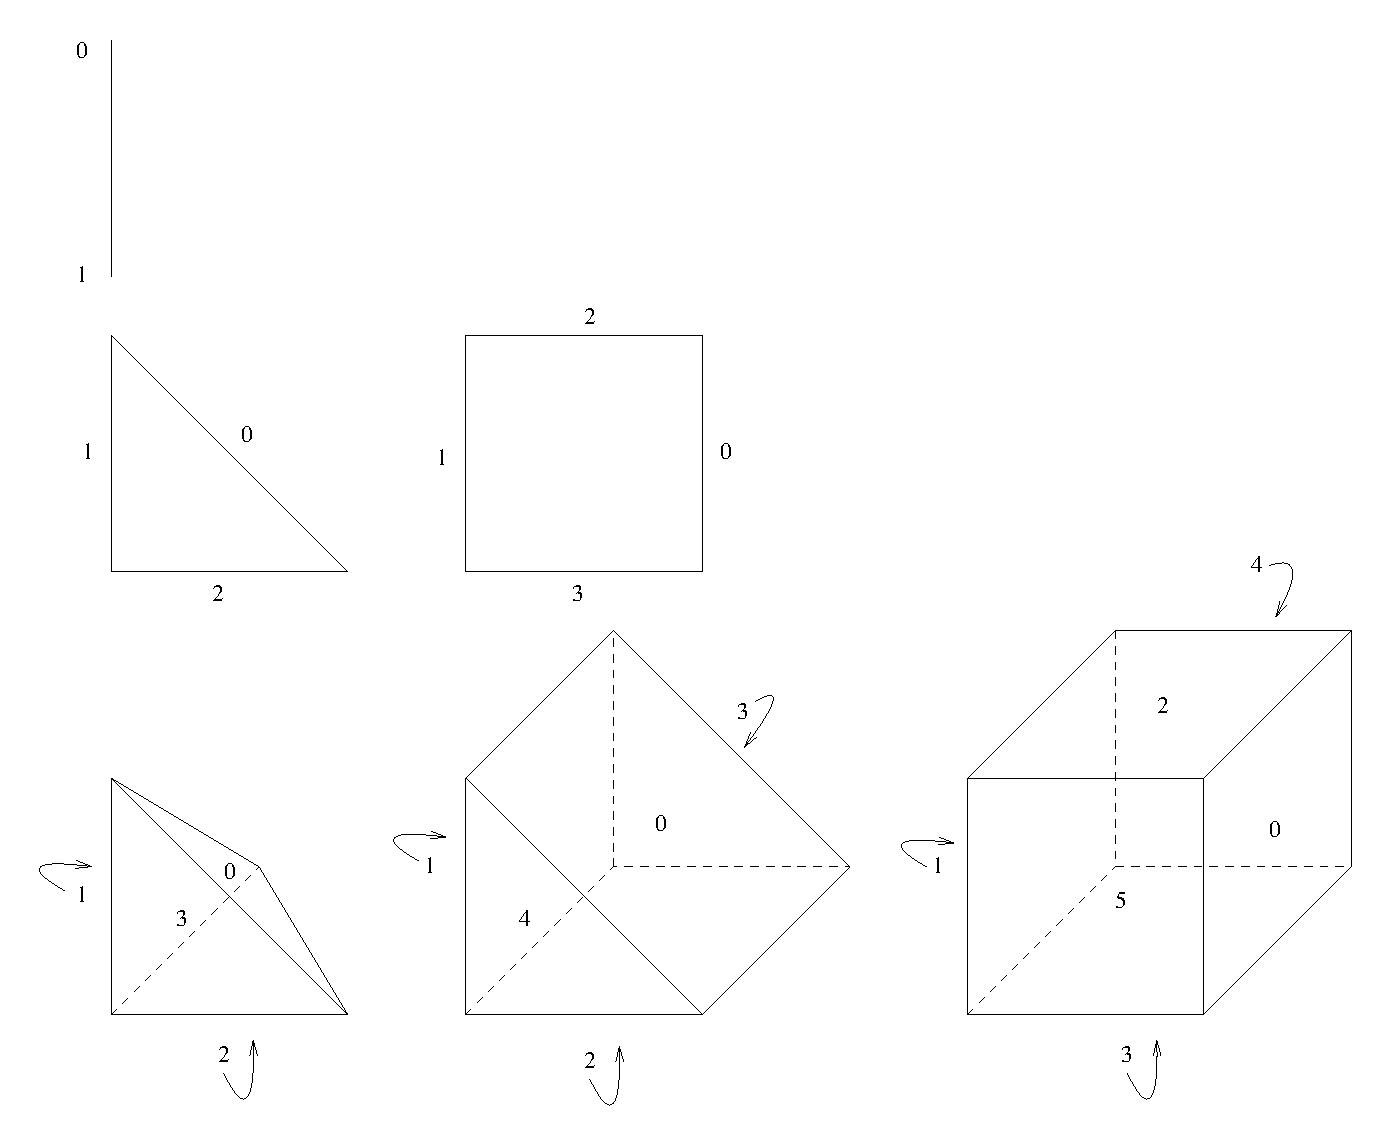
\includegraphics[width=15cm,angle=0]{getfemuserelemf}}
    \htmlonly{\htmlimg{getfemuserelemf.png}{faces numeration for usual elements}}
  \end{center}
  \caption{ \it faces numeration for usual elements }
  \label{fig:elemf}
\end{figure}

\subsection{Save, load and draw meshes}

In \filename{getfem\_mesh.h}, two methods are defined to load meshes from file and write meshes to a file. \\[0.5cm]
\index{GETFEM!mesh.write\_to\_file(name)}
\index{GETFEM!mesh.read\_from\_file(name)}
\begin{ctableau}{|m{0.4\linewidth}|m{0.55\linewidth}|}{ll}\hline

  \cpp{mesh.write\_to\_file(const std::string \&name)} & save the mesh into a file.\\ \hline

  \cpp{mesh.read\_from\_file(const std::string \&name)} & load the mesh from a file.\\ \hline

\end{ctableau}

A little tool allows to display a mesh using Gnuplot (and Perl). This tool is present in the directory \filename{contrib/} and of course you need to have a working distribution of Gnuplot installed on your system. This little tool is built when you execute a {\tt make} instruction on the root directory of \gf . So, if \gf  is normally installed on your system, you can change your current directory to \filename{contrib/} and execute the command \\[0.5cm]
{\tt draw\_mesh filename.mesh} \\[0.5cm]
where {\tt filename.mesh} is the file containing the mesh. This works only for meshes whose principal dimension is between 1 and 3. Examples of mesh files are also provided into the directory \filename{contrib/} to test the program.

\subsection{example}

The following is an example of how to load a mesh and extract information on it.
\begin{cppcode}
  \#include <getfem\_mesh.h>
  
  getfem::getfem\_mesh mesh; 
  
  int main(int argc, char *argv[]) \{ 
    try \{ 
     
      // read the mesh from the file name given by the first argument 
      mesh.read\_from\_file(std::string(argv[0])); 
     
      // List all the convexes
      dal::bit\_vector nn = mesh.convex\_index(); 
      bgeot::size\_type i; 
      for (i << nn; i != bgeot::size\_type(-1); i << nn) \{
        cout << "Convex of index " << i << endl; 
        bgeot::pconvex\_structure cvs =  mesh.structure\_of\_convex(i); 
        cout << "Number of vertices : " << cvs->nb\_points() << endl; 
        cout << "Number of faces : " << cvs->nb\_faces() << endl;
        for (bgeot::size\_type f = 0; f < cvs->nb\_faces(); ++f) \{
          cout << "face " << f << " has " << cvs->nb\_points\_of\_face(f); 
          cout << " vertices with local indexes : "; 
          for (bgeot::size\_type k = 0; k < cvs->nb\_points\_of\_face(f); ++k) 
          cout << cvs->ind\_points\_of\_face(f)[k] << " "; 
          cout << " and global indexes : ";
          for (bgeot::size\_type k = 0; k < cvs->nb\_points\_of\_face(f); ++k) 
            cout << mesh.ind\_points\_of\_convex(i)(cvs->ind\_points\_of\_face(f)[k]) << " ";
        \}
     \}
     
   \} DAL\_STANDARD\_CATCH\_ERROR; // catches standard errors
 \}
\end{cppcode}

\section{Select finite element and integration methods}

\index{GETFEM!getfem::mesh\_fem}
In order to define a complete finite element procedure on a mesh, the structure \cpp{getfem::mesh\_fem} is defined in the file \cpp{getfem\_mesh\_fem.h}. Basically, this structure describe the finite element method on each element of the mesh, and can store information about boundary structure. It is possible to have an arbitrary number of finite element description for a single mesh. This is particularly necessary for mixed methods, but also to describe different data on the same mesh. One can instantiate a \cpp{getfem::mesh\_fem} object as follows\\[0.5cm]
\cpp{getfem::mesh\_fem mef(mesh); }\\[0.5cm]
where \cpp{mesh} is an already existing mesh. The structure will be linked to this mesh and will react when modifications will be done on it. \\[0.5cm]
It is possible to specify element by element the finite element method, so that element of mixed types can be treated, even if the dimensions are different. For usual elements, the connection between two elements is done when the two elements are compatibles (same degrees of freedom on the common face). A numeration of the degrees of freedom is automatically done with a Cuthill Mc Kee like algorithm. You have to keep in mind that there is absolutely no connection between the numeration of vertices of the mesh and the numeration of the degrees of freedom. Every \cpp{getfem::mesh\_fem} object has its own numeration. \\[0.5cm]
To select a particular finite element method on a given element, one can use \\[0.5cm]
\index{GETFEM!mef.set\_finite\_element(i, ppf, ppi)}
\cpp{mef.set\_finite\_element(i, ppf, ppi); }\\[0.5cm]
where \cpp{i} is the index of the element, \cpp{ppf} is the descriptor of the finite element method, and \cpp{ppi} is the descriptor of the integration method. The list of all available descriptors of finite element methods is in the file \filename{getfem\_fem.h}. A short description is also given in \cite{BASCOMP}. The list of all available descriptors of integration methods is in the file \filename{getfem\_integration.h}. \\[0.5cm]
Descriptors for finite element methods and integration methods are available thanks to the two follofing functions\\[0.5cm]
\index{GETFEM!getfem::fem\_descriptor("name")}
\index{GETFEM!getfem::nt\_method\_descriptor("name")}
\begin{cppcode}
  ppf = getfem::fem\_descriptor("name of method");
  ppi = getfem::int\_method\_descriptor("name of method");
\end{cppcode}
where \cpp{"name of method"} is to be chosen among the existing methods.
A name of a method can be retrieved thanks to the following functions\\[0.5cm]
\begin{cppcode}
  std::string femname = getfem::name\_of\_fem(ppf); 
  std::string im\_name = getfem::name\_of\_int\_method(ppi);
\end{cppcode}
A non exhautive list (see \cite{FEMLIST} for exhaustive lists) of finite element methods is given by
\begin{center} \begin{tabular}{|m{0.55\linewidth}|m{0.4\linewidth}|} \hline
{\tt getfem::ppolyfem getfem::PK\_fem(n, k)} & Classical $P_K$ methods on simplexes of dimension  {\tt n} with degree {\tt k} polynomials.\\ \hline
{\tt getfem::ppolyfem getfem::QK\_fem(n, k)} & Classical $Q_K$ methods on parallelepiped of dimension {\tt n}. Tensorial product of degree {\tt k} $P_K$ method on the segment. \\ \hline
{\tt getfem::ppolyfem getfem::PK\_prism\_fem(n, k)} & Classical methods on prism of dimension {\tt n}. Tensorial product of two degree {\tt k} $P_K$ method. \\ \hline
{\tt getfem::ppolyfem getfem::product\_fem( ppolyfem\;a, ppolyfem b)} & Tensorial product of the two polynomial finite element method {\tt a} and {\tt b}. \\ \hline
{\tt getfem::ppolyfem $\;$ getfem::P1\_nonconforming\_fem()} & Non conforming $P_1$ method on triangles. \\ \hline
\end{tabular} \end{center}

Examples of exact integration methods:
\begin{center} \begin{tabular}{|m{0.55\linewidth}|m{0.4\linewidth}|} \hline
{\tt "IM\_EXACT\_SIMPLEX(n)"} & Description of the exact integration of polynomials on the simplex of reference of dimension {\tt n}. \\ \hline
\end{tabular}  
\begin{tabular}{|m{0.55\linewidth}|m{0.4\linewidth}|} \hline
{\tt "IM\_PRODUCT(a, b)"} & Description of the exact integration on the convex which is the direct product of the convex in {\tt a} and in {\tt b}.\\ \hline
\end{tabular}  
\begin{tabular}{|m{0.55\linewidth}|m{0.4\linewidth}|} \hline
{\tt "IM\_EXACT\_PARALLELEPIPED(n)"} & Description of the exact integration of polynomials on the parallelepiped of reference of dimension {\tt n}\\ \hline
\end{tabular}  
\begin{tabular}{|m{0.55\linewidth}|m{0.4\linewidth}|} \hline
{\tt "IM\_EXACT\_PRISM(n)"} & Description of the exact integration of polynomials on the prism of reference of dimension {\tt n}\\ \hline
\end{tabular} \end{center}

Examples of approximated integration methods:
\begin{center} \begin{tabular}{|m{0.55\linewidth}|m{0.4\linewidth}|} \hline
{\tt "IM\_GAUSS1D(k)" } & Description of the Gauss integration on a segment of order {\tt k}. \\ \hline
\end{tabular}  
\begin{tabular}{|m{0.55\linewidth}|m{0.4\linewidth}|} \hline
{\tt "IM\_NC(n,k)"} & Description of the integration on a simplex of reference of dimension {\tt n} for polynomials of degree {\tt k} with the Newton Cotes method (based on Lagrange interpolation).\\ \hline
\end{tabular}  
\begin{tabular}{|m{0.55\linewidth}|m{0.4\linewidth}|} \hline
{\tt "IM\_PRODUCT(a,b)"} & Build a method doing the direct product of methods {\tt a} and {\tt b}. \\ \hline
\end{tabular}  
\begin{tabular}{|m{0.55\linewidth}|m{0.4\linewidth}|} \hline
{\tt "IM\_TRIANGLE(2)"} & Integration on a triangle of order 2 with 3 points. \\ \hline
\end{tabular}
\begin{tabular}{|m{0.55\linewidth}|m{0.4\linewidth}|} \hline
{\tt "IM\_TRIANGLE(7)"} & Integration on a triangle of order 7 with 13 points. \\ \hline
\end{tabular} 
\begin{tabular}{|m{0.55\linewidth}|m{0.4\linewidth}|} \hline
{\tt "IM\_QUAD(2)"} & Integration on quadrilaterals of order 2 with 3 points. \\ \hline
\end{tabular}
\begin{tabular}{|m{0.55\linewidth}|m{0.4\linewidth}|} \hline
{\tt "IM\_TETRAHEDRON(5)"} & Integration on a tetrahedron of order 5 with 15 points. \\ \hline
\end{tabular} \end{center}


For instance if one needs to have a description of a $P_1$ finite element method on a triangle with an exact integration, the way to set it is
\begin{cppcode}
 mef.set\_finite\_element(i, getfem::fem\_descriptor("FEM\_PK(2, 1)"),
                        getfem::int\_method\_descriptor("IM\_EXACT\_SIMPLEX(2)"));
\end{cppcode}
where \cpp{i} is still the index of the triangle. It is also possible to select a particular method directly on a set of element, passing to \cpp{mef.set\_finite\_element} a \cpp{dal::bit\_vector} instead of a single index. For instance
\begin{cppcode}
 mef.set\_finite\_element(mesh.convex\_index(), getfem::fem\_descriptor("FEM\_PK(2, 1)"),
                        getfem::int\_method\_descriptor("IM\_EXACT\_SIMPLEX(2)"));
\end{cppcode}
selects the method on all the elements of the mesh.\\[0.5cm]
IMPORTANT: If the finite element represents an unknown for a vectorial problem (such as linear elasticity), one should use
\cpp{mef.set\_qdim(Q)}\\[0.5cm]
to set the target dimension (see
\cite{BASCOMP} for the definition of the target dimension $Q$)\\[0.5cm]
If the target dimension $Q$ is set to a value different of $1$, the
scalar FEMs (such as $P_k$ fems etc.) are automatically
``vectorized'', i.e. each scalar degree of freedom is duplicated $Q$
times, from the \cpp{mesh\_fem} object point of vue. To sum it up,
\begin{itemize}
\item if the fem of the $ith$ element is a real vector FEMs, \cpp{mef.get\_qdim() == mef.fem\_of\_element(i)->target\_dim()} \\ and\\ \cpp{
    mef.nb\_dof\_of\_element(i) == mef.fem\_of\_element(i).nb\_dof()}.
\item if the fem has a \cpp{target\_dim} equal to $1$, \cpp{mef.nb\_dof\_of\_element(i) == mef.get\_qdim()*mef.fem\_of\_element(i).nb\_dof()}.
\end{itemize}

Once a finite element method is defined on a mesh, it is possible to obtain information on it with the following methods (the list is not exhaustive).\\[0.5cm]
\begin{center} \texonly{\begin{tabular}{|m{0.4\linewidth}|m{0.55\linewidth}|} \hline}\htmlonly{\xmlattributes*{table}{border}\begin{tabular}{l|l}}

  \cpp{mef.convex\_index()} & Set of indexes (a \cpp{dal::bit\_vector}) on which a finite element method is defined.  \\ \hline

  \cpp{mef.linked\_mesh()} & gives a reference to the linked mesh.  \\ \hline

  \cpp{mef.fem\_of\_element(i)} & gives a descriptor on the finite element method defined on element of index \cpp{i}.  \\ \hline

  \cpp{mef.int\_method\_of\_element(i)} & gives a descriptor on the integration method defined on element of index \cpp{i}.  \\ \hline

  \cpp{mef.nb\_dof\_of\_element(i)} & gives the number of degrees of freedom on the element of index \cpp{i}.  \\ \hline

  \cpp{mef.ind\_dof\_of\_element(i)} & gives a container (an array) with all the global indexes of the degrees of freedom of element of index \cpp{i}.  \\ \hline

  \cpp{mef.point\_of\_dof(i, j)} & gives a \cpp{bgeot::base\_node} which represents the point associated with the dof of local index \cpp{j} on element of index \cpp{i}.  \\ \hline

  \cpp{mef.point\_of\_dof(j)} & gives a \cpp{bgeot::base\_node} which represents the point associated with the dof of global index \cpp{j}.  \\ \hline

  \cpp{mef.reference\_point\_of\_dof(i, j)} & gives a \cpp{bgeot::base\_node} which represents the point associated with the dof of local index \cpp{j} on element of index \cpp{i} in the coordinates of the reference element.  \\ \hline

  \cpp{mef.first\_convex\_of\_dof(j)} & gives the index of the first element on which the degree of freedom of global index \cpp{j} is defined.  \\ \hline
  
  \cpp{mef.nb\_dof()} & gives the total number of different degrees of freedom.  \\ \hline

  \cpp{mef.get_qdim()} & gives the target dimension \cpp{Q}.  \\ \hline

  \cpp{mef.clear()} & Clear the structure, no finite element method is still defined.  \\ \hline

  \cpp{mef.add\_boundary\_elt(b, c, f)} & Add a face to a description of a boundary. Add the face \cpp{f} of the element of index \cpp{c} to the boundary of index \cpp{b}.  \\ \hline
  
  \cpp{mef.sup\_boundary\_elt(b, c, f)} & remove a face to a description of a boundary. remove the face \cpp{f} of the element of index \cpp{c} to the boundary of index \cpp{b}.  \\ \hline
\end{tabular} \end{center}

\begin{center} \begin{tabular}{|m{0.4\linewidth}|m{0.55\linewidth}|} \hline
  
  \cpp{mef.is\_convex\_on\_boundary(c, b)} & return either or not the convex of index \cpp{c}  has a face on the boundary of index \cpp{b}.  \\ \hline
  
  \cpp{mef.convex\_on\_boundary(b)} & return a \cpp{dal::bit\_vector} containing all the indexes of all the elements having at least one face on boundary of index \cpp{b}.  \\ \hline

  \cpp{mef.faces\_of\_convex\_on\_boundary(c, b) } & return a \cpp{dal::bit\_vector} containing all the local indexes of faces of the element of index \cpp{c} which contained on the boundary of index \cpp{b}.  \\ \hline

  \cpp{mef.sup\_boundary(b) } & remove the boundary of index \cpp{b}.  \\ \hline

\end{tabular} \end{center}

\section{Linear algebra procedures}
\index{GMM| Generic Matrix Methods library, }
\index{ITL| Iterative Template Library, }
\index{MTL| Matrix Template Library, }
Assembling procedures, especially for Dirichlet boundary conditions need some basic linear algebra computation. In order to make \gf  independent of any matrix library, it contains one called GMM (for Generic Matrix Methods). Theoretically, this library provides a mean to interface any other matrix library. If you want to use your own matrix library, you have just to write some ``traits'' objects. GMM provide also some basic types of sparse and plain matrices and vectors and basic operations on them (copy, addition, multiplication, sub vector and matrices, solvers ... ). The syntax of GMM is very closed to MTL and ITL (see http://www.osl.iu.edu/research/mtl/). Escpecially, the code for iterative solvers has been copied from ITL. The performance of GMM is very closed to the one of MTL, sometime slightly better. The difference between GMM and MTL is that basically GMM has been written to be able to interface other libraries and gives an access to sub matrices and sub vectors in all cases. Also some optimizations has been made for matrix-matrix multiplication, usage of reference has been somewhat cleared, const qualifier usage is clarified, and we hope it is somewhat easier to use than MTL. The bad news is that some fonctionnalities have not yet been imported.\\

To use GMM you have to include the file \filename{gmm.h}.

\subsection{Matrix and Vector type provided by GMM}

\subsubsection{plain vectors}
\index{GMM! std::vector<T>}
\index{BGEOT! bgeot::vsvector<T>}
GMM interfaces directly \cpp{std::vector<T>} so you can used it as your basic plain vector type. You can use also \cpp{bgeot::vsvector<T>} form \cpp{bgeot} library. If you need to interface another type of plain vector you can see in \cpp{gmm_interface.h} some examples.\\

\cpp{vect_size(V)} gives the size of a vector.

\subsubsection{sparse vectors}
\index{GMM! gmm::wsvector<T>}
\index{GMM! gmm::rsvector<T>}
GMM provides two types of sparse vectors: \cpp{gmm::wsvector<T>} and \cpp{gmm::rsvector<T>}. \cpp{gmm::wsvector<T>} is optimized for write operations and \cpp{gmm::rsvector<T>} is optimized for read operations. It should be appropriate to use \cpp{gmm::wsvector<T>} for assembling procedures and then to copy the vector in a \cpp{gmm::rsvector<T>} for the solvers. The initialization is
\begin{cppcode}
  gmm::rsvector<double> V(s);
\end{cppcode}
where \cpp{s} is the size. For all copy operations use\\[0.2cm]
\begin{tt}
  gmm::copy (V, W);
\end{tt}\\[0.2cm]
instead of \cpp{W = V} which is not always supported.
\index{GMM! gmm::vect_size(V)}
\cpp{gmm::vect_size(V)} gives the size of a vector.

\subsubsection{matrices}
\index{GMM! gmm::row_matrix<VECT>}
\index{GMM! gmm::col_matrix<VECT>}
\index{BGEOT! bgeot::vsmatrix<T>}
GMM provides two types of matrices: \cpp{gmm::row_matrix<VECT>} and \cpp{gmm::col_matrix<VECT>} where \cpp{VECT} should be a valid (i.e. interfaced) vector type.
Those two type of matrices store an array of \cpp{VECT} so the memory is not contiguous. You can also use \cpp{bgeot::vsmatrix<T>} from \cpp{bgeot} library which is a plain matrix with a contiguous memory and fortran type access (column major). Initialisations are
\begin{cppcode}
  gmm::row_matrix< std::vector<double> > M1(10, 10);  // plain row matrix
  gmm::col_matrix< gmm::wsvector<double> > M2(5, 20); // sparse column matrix
  bgeot::vsmatrix<double> M3(4, 5); // plain column and row matrix
\end{cppcode}
Of course \cpp{gmm::row_matrix<VECT>} is a row matrix and it is impossible to access to a particular column of this matrix. \cpp{bgeot::vsmatrix<T>} is considered as a column and row matrix (column prefered) and you can access both to the columns and rows.
\index{GMM! gmm::mat_nrows(M)}
\index{GMM! gmm::mat_ncols(M)}\\

\cpp{gmm::mat_nrows(M)} gives the number of rows of a matrix and \cpp{gmm::mat_ncols(M)} the number of columns.


\subsection{sub-vectors and sub-matrices}
\index{GMM! gmm::sub_interval(first, length)}
It is possible to obtain any sub-vector or sub-matrix of a fully interfaced object. There are three type of sub indexes.
\begin{cppcode}
  gmm::sub_interval(first, length);
\end{cppcode}
represents an interval whose first index is \cpp{first} and length is \cpp{lenght} ( for instance \cpp{gmm::sub_interval(10, 3);} represents the indexes \cpp{\{10, 11, 12\} }).
\index{GMM! gmm::sub_slice(first, length, step)}
\begin{cppcode}
  gmm::sub_slice(first, length, step);
\end{cppcode}
represents also an interval in which one index over \cpp{step} is taken. ( for instance \cpp{gmm::sub_slice(10, 3, 2);} represents the indexes \cpp{\{10, 12, 14\} })
\begin{cppcode}
  gmm::sub_index(CONT c);
\end{cppcode}
represents the sub-index which is the collection of index contained in the container \cpp{c}. For instance
\index{GMM! gmm::sub_index(c)}
\begin{cppcode}
  std::vector<size_t> c(3);
  c[0] = 1; c[1] = 3; c[2] = 16;
  gmm::sub_index(c);
\end{cppcode}
represents the indexes \cpp{\{1, 3, 16\} }. \\

\index{GMM! gmm::sub_vector(V, subi)}
Now \cpp{gmm::sub_vector(V, subi)} gives a reference to a sub-vector:
\begin{cppcode}
  gmm::vsvector<double> V(10);
  V[5] = 3.0;
  std::cout << gmm::sub_vector(V, gmm::sub_interval(2, 3)) << std::endl;  
\end{cppcode}
prints to the standard output \cpp{V[2], V[3]} and \cpp{V[4]}.\\

\index{GMM! gmm::sub_matrix(V, subi1, subi2)}
\cpp{gmm::sub_matrix(V, subi1, subi2)} gives a reference to a sub-matrix. For instance:
\begin{cppcode}
  gmm::col_matrix< gmm::wsvector<double> > M(5, 20);
  M(3, 2) = 5.0;
  std::cout << gmm::sub_matrix(M, gmm::sub_interval(2, 3), gmm::sub_interval(2, 3))
            << std::endl;  
\end{cppcode}
prints to the output a sub-matrix. If the two sub-indexes are equal, it is possible to ommit the second. For instance:
\begin{cppcode}
  gmm::col_matrix< gmm::wsvector<double> > M(5, 20);
  M(3, 2) = 5.0;
  std::cout << gmm::sub_matrix(V, gmm::sub_interval(2, 3)) << std::endl;  
\end{cppcode}

\subsubsection{row and column of a matrix}
\index{GMM! gmm::mat_row(M, i)}
\index{GMM! gmm::mat_col(M, i)}
\index{GMM! gmm::mat_const_row(M, i)}
\index{GMM! gmm::mat_const_col(M, i)}
\cpp{gmm::mat_row(M, i)} gives a (possibly writable) reference to the row \cpp{i} of matrix \cpp{M}, and \cpp{gmm::mat_col(M, i)}  gives a (possibly writable) reference to the column \cpp{i}. It is not possible to access to the rows if \cpp{M} is a column matrix and to the columns if it is a row matrix. It is possible to use \cpp{gmm::mat_const_row(M, i)} and \cpp{gmm::mat_const_col(M, i)} to have constant references.


\subsection{Basic linear algebra operations}
The same choice has been made as in MTL to provide basic operations as functions not as operators. The advantages are that it is clearer to see where are the linear algebra operations in the program and the programmation of optimized basic linear operations is greatly simpler.

\subsubsection{write}
\index{GMM! gmm::write}
\begin{cppcode}
  gmm::write(o, V); gmm::write(o, M);
\end{cppcode}
print the vector or the matrix to the output stream o. For instance
\begin{cppcode}
  gmm::write(cout, V); gmm::write(cout, M);
\end{cppcode}
write them on the standard output.
Most of the time it is also possible to use simply
\begin{cppcode}
  std::cout << V << std::endl; std::cout << M << std::endl;
\end{cppcode}

\subsubsection{clear}
\index{GMM! gmm::clear}
\begin{cppcode}
  gmm::clear(V); gmm::clear(M);
\end{cppcode}
set to zero all the components of a vector or a matrix.

\subsubsection{scale}
\index{GMM! gmm::scale}
\index{GMM! gmm::scaled}
\cpp{gmm::scale} is used to multiply a vector or a matrix with a scalar factor.
\begin{cppcode}
  gmm::scale(V, 10.0);  // V * 10.0 ---> V
\end{cppcode}
If one not needs to multiply the vector but wants to use the multiplied vector in an expression  \cpp{gmm::scaled } gives a reference to a multiplied vector. This is only a reference, no operation is made until this reference is used somewhere. For instance
\begin{cppcode}
  std::cout << gmm::scaled(V, 10.0) << std::endl;
\end{cppcode}
print to the standard output the vector \cpp{V} multiplied by \cpp{10.0} without changing \cpp{V}.

\subsubsection{transposition}
\index{GMM! gmm::transposed}
\cpp{gmm::transposed(M) } gives a reference on the transposed matrix of \cpp{M}.


\subsubsection{add}
\index{GMM! gmm::add}
addition of vectors or matrices. It is alway possible to mixe different type of vector or matrices in the operations. The following operations are valid:
\begin{cppcode}
  std::vector<double> V1(10);
  gmm::wsvector<double> V2(10);
  gmm::clear(V1);
  ...
  gmm::add(V1, V2); // V1 + V2 --> V2
  cout << V2;

  gmm::add(V1, gmm::scaled(V2, -2.0), V2); // V1 - 2.0 * V2 --> V2
  cout << V2;

  gmm::row_matrix< std::vector<double> > M1(10, 10);
  gmm::col_matrix< gmm::wsvector<double> > M2(1000, 1000);

  // M1 + (sub matrix of M2) ---> (sub matrix of M2)
  gmm::add(M1, gmm::sub_matrix(M2, gmm::sub_interval(4,10)));
\end{cppcode}

\subsubsection{mult}
\index{GMM! gmm::mult}
Matrix-vector or matrix-matrix multiplication . The following operations are valid:
\begin{cppcode}
  std::vector<double> V1(10);
  gmm::wsvector<double> V2(10);
  ...
  gmm::row_matrix< std::vector<double> > M1(10, 10);
  ...

  gmm::mult(M1, V2, V1);  // M1 * V2 --> V1

  gmm::mult(M1, V2, V2, V1);  // M1 * V2 + V2 --> V1

  gmm::mult(M1, gmm::scaled(V2, -1.0), V2, V1);  // M1 * (-V2) + V2 --> V1

  gmm::col_matrix< gmm::wsvector<double> > M2(10, 10);
  gmm::col_matrix< gmm::vsvector<double> > M3(10, 10);
  ...
  
  gmm::mult(M1, M2, M3); // M1 * M2 ---> M3
  
  gmm::mult(gmm::sub_matrix(M1, sub_interval(0, 3)),
            gmm::sub_matrix(M2, sub_interval(4, 3)),
            gmm::sub_matrix(M3, sub_interval(2, 3)));

\end{cppcode}

\subsubsection{clean}
\index{GMM! gmm::clean}
 \cpp{gmm::clean(V, 1E-12); } set to zero all the components of \cpp{V} whose modulous is less or equal to \cpp{ 1E-12}. Works also for matrices.

\subsubsection{norms}
\index{GMM! gmm::vect_norm1(V)}
\index{GMM! gmm::vect_norm2(V)}
\index{GMM! gmm::vect_inf(V)}
  for vectors only, \cpp{gmm::vect_norm1(V)} gives the sum of modulous of the components of \cpp{V}.\\
\cpp{gmm::vect_norm2(V)} is the euclidian norm of \cpp{V} and \cpp{gmm::vect_inf(V)} the infinity norm of \cpp{V}.

\subsubsection{scalar product} 
\index{GMM! gmm::vect_sp(V1, V2)}
  for vectors only, \cpp{gmm::vect_sp(V1, V2); } gives the scalar product between \cpp{V1} and \cpp{V2}.


\subsection{solvers}
Most of the solvers provided in GMM come form ITL with slight modifications.

\subsubsection{iterations}
\index{GMM! gmm::iteration}
  The iteration object of GMM is a modification of the one in ITL. This is not a template type as in ITL. Preconditionners has not been yet fully implemented in GMM, so for the moment it is only possible to use precondionners whose inverse is represented by a matrix. 

The simplest initialisation is
\begin{cppcode}
  gmm::iteration iter(2.0E-10);
\end{cppcode}
where \cpp{2.0E-10} is the (relative) residual to be obtained to have the convergence.
Some possibilities :
\begin{cppcode}
  iter.set_noisy(n) // n = 0 : no output
                    // n = 1 : output of iterations on the standard output
                    // n = 2 : output of iterations and sub-iterations 
                    //         on the standard output
                    // ...
  iter.get_iteration() // after a computation, gives the number of
                       // iterations made.
  iter.converged()     // true if the method converged.
  iter.set_maxiter(n)  // Set the maximum of iterations.
                       // A solver stops if the maximum of iteration is 
                       // reached, iter.converged() is then false.
\end{cppcode}

\subsubsection{various solvers}
To solve linear systems.
\index{GMM! gmm::cg}
\index{GMM! gmm::bicgstab}
\index{GMM! gmm::gmres}
\index{GMM! gmm::qmr}
\index{GMM! gmm::cheby}
\index{GMM! gmm::constrained_cg}
\begin{cppcode}
  gmm::row_matrix< std::vector<double> > A(10, 10);  // The matrix
  std::vector<double> B(10); // Right hand side
  std::vector<double> X(10); // Unknown
  gmm::identity_matrix PS;   // Optionnal scalar product for cg
  gmm::identity_matrix PR;   // Optionnal preconditionner
  ...
  gmm::iteration iter(10E-9);// Iteration object with the max residu
  size_t restart = 50;       // restart parameter for GMRES
  
  gmm::cg(A, X, B, PS, PR, iter); // Conjugate gradient

  gmm::bicgstab(A, X, B, PR, iter); // BICGSTAB BiConjugate Gradient Stabilized

  gmm::gmres(A, X, B, PR, restart, iter) // GMRES generalized minimum residual

  gmm::qmr(A, X, B, PR, PR, iter) // Quasi-Minimal Residual method.

  gmm::cheby(A, X, B, PR, iter) // Preconditioned Chebyshev Method.
\end{cppcode}

The solver \cpp{gmm::constrained_cg(A, C, X, B, PS, PR, iter);} solve a system with linear constaints, \cpp{C} is a matrix which represents the constraints.

\subsection{deeper inside GMM}

\subsubsection{iterators on vectors and matrices}
... to be done (see \filename{gmm_blas.h}).

\subsubsection{Specify and optimize a particular algorithm}
... to be done

\subsubsection{How to interface a new vector}
... to be done (see examples in \filename{gmm_interface.h}).

\subsubsection{How to interface a new matrix}
... to be done (see examples in \filename{gmm_interface.h}).

\section{Standard assembling procedures}

Procedures defined in the file \filename{getfem\_assembling.h} allow to assemble stiffness matrices, mass matrices and boundary conditions for a few amount of classical partial differential equation problems. All the procedures have vectors and matrices template parameters in order to be used with any matrix library.

\subsection{Laplacian (Poisson) problem}
\index{laplacian}
\index{Poisson problem}

An assembling procedure is defined to solve the problem
\texonly{\begin{eqnarray*}
  \Div (a(x)\ \Grad u(x)) = f(x), \ \ \text{in $\Omega$}, \\
  u(x) = U(x),  \ \ \text{on $\Gamma_{_D}$}, \\
  \Frac{\partial u}{\partial \bf n} = F(x),  \ \ \text{ on $\Gamma_{_N}$}, 
\end{eqnarray*}
}\htmlonly{
  \begin{equation*}
    \Div (a(x)\ \Grad u(x)) = f(x), \ \ \text{in $\Omega$},
  \end{equation*}
}
where $\Omega$ is an open domain of arbitrary dimension, $\Gamma_{_D}$ and $\Gamma_{_N}$ are parts of the boundary of $\Omega$, $u(x)$ is the unknown, $a(x)$ is a given coefficient, $f(x)$ is a given source term, $U(x)$ the prescribed value of $u(x)$ on $\Gamma_{_D}$ and $F(x)$ is the prescribed normal derivative of $u(x)$ on $\Gamma_{_N}$.
The function to be called to assemble the stiffness matrix is\\[0.5cm]
\index{GETFEM!getfem::asm\_stiffness\_matrix\_for\_laplacian}
\cpp{getfem::asm\_stiffness\_matrix\_for\_laplacian(SM, mef1, mef2, A);} \\[0.5cm]
where \cpp{SM} is a matrix of any type having the right dimension (i.e. \cpp{me1.nb\_dof()}), \cpp{mef1} is a variable of type \cpp{getfem::mesh\_fem} and should define the finite element method for the solution, \cpp{mef2}  is a variable of type \cpp{getfem::mesh\_fem} (possibly equal to \cpp{mef1}) describing the finite element method on which the coefficient $a(x)$ is defined, and \cpp{A} is the vector of the values of this coefficient on each degree of freedom of \cpp{mef2}. Both should use the same mesh. It is important to pay attention to the fact that the integration methods used to compute the elementary matrices is the ones declared in \cpp{mef1}. This integration method have to be chosen of sufficient order. The order has to be determined considering the degrees of element in \cpp{mef1}, in \cpp{mef2} and the geometric transformations for non-linear cases. Integration methods defined in \cpp{mef2} are ignored.\\[0.5cm]
To assemble the source term, the  function to be called is\\[0.5cm]
\index{GETFEM!getfem::asm\_source\_term}
\cpp{getfem::asm\_source\_term(B, mef1, mef2, V);} \\[0.5cm]
where \cpp{B} is a vector of any type having the right dimension (still \cpp{me1.nb\_dof()}), \cpp{mef2}  is a variable of type \cpp{getfem::mesh\_fem} (possibly equal to \cpp{mef1}) describing the finite element method on which $f(x)$ is defined, \cpp{V} is the vector of the values of $f(x)$ on each degree of freedom of \cpp{mef2}.\\[0.5cm]
For the Neumann condition on $\Gamma_{_N}$, the same function\\[0.5cm]
\cpp{getfem::asm\_source\_term(B, mef1, mef2, V, nbound);} \\[0.5cm]
is used again, but an additionnal argument has been added: \cpp{nbound} is the index of the boundary in \cpp{mef1} (see previous section on how to describe a boundary) where the Neumann condition is applied. Hence the assembly is done on the indicated boundary, and no more on the whole domain. \cpp{mef2}  is a variable of type \cpp{getfem::mesh\_fem} describing the finite element method on which $F(x)$ is defined, \cpp{V} is the vector of the values of $F(x)$ on each degree of freedom of \cpp{mef2}.\\[0.5cm]
there is two manner to take into account the Dirichlet condition on $\Gamma_{_D}$, changing the linear system or explicitly reduce to the kernel of the Dirichlet condition. For the first manner, the following function is defined \\[0.5cm]
\index{GETFEM!getfem::assembling\_Dirichlet\_condition}
\cpp{getfem::assembling\_Dirichlet\_condition(SM, B, mef1, nbound, V, N);} \\[0.5cm]
where \cpp{nbound} is the index of the boundary in \cpp{mef1} where the Dirichlet condition is applied, \cpp{V} is the vector of the values of $U(x)$ on each degree of freedom of \cpp{mef1} and \cpp{N} is the dimension for vectorial problems (should be \cpp{1} for scalar problems). This operation should be the last one because it transform the stiffness matrix \cpp{SM}. It works only for Lagrange elements. At the end, one obtains the discrete system
\begin{equation*} [SM] U = B, \end{equation*}
where $U$ is the discrete unknown.\\[0.5cm]

\T \newcommand{\tildeH}{\tilde{H}}
\W \newcommand{\tildeH}{HH}
\T \newcommand{\tildeR}{\tilde{R}}
\W \newcommand{\tildeR}{RR}
\T \newcommand{\tildeR}{\tilde{N}}
\W \newcommand{\tildeR}{NN}


For the second manner, one should use\\[0.5cm]
\index{GETFEM!getfem::asm\_dirichlet\_constraints}
\cpp{getfem::asm\_dirichlet\_constraints($\tildeH$, $\tildeR$, mf\_u, mf\_rh,$H$, $R$, nbound)}.\\[0.5cm]
See the Dirichlet condition as a general linear constraint that must
satisfy the solution $u$. This function does the assembly of 
Dirichlet conditions of type $h(x).u(x) = r(x)$ where h is a small square matrix
  (of any rank) whose size is equal to \cpp{gf_mesh_fem_get(mf_u,'Qdim')}.
  This matrix is stored in \cpp{H}, one column per dof in
  \cpp{mf\_rh}, each column containing the values of the matrix $h$ stored
  in Fortran order: for example \cpp{Hd(:,j)}$ = [h_{11}(x_j) h_{21}(x_j) h_{12}(x_j) h_{22}(x_j)]$ if $u$ is a 2D vector field.
  Of course, if the unknown $u$ is a scalar field, \cpp{H} is just a row vector

Here, $H$ is a (sparse) matrix, with \cpp{mf\_rh.nb\_dof()} columns, and $n_c$ lines, where $n_c$ is the number
of constraints. Hence $u$ must satisfy $Hu=R$, which is expressed on
$mf\_rh$ (hopefully Lagrangian). This function just assemble these
constraints into a new linear system $\tildeH u=\tildeR$, doing some
additional simplification in order to obtain a ``simple'' constraints
matrix.  \index{GETFEM!getfem::Dirichlet\_nullspace} Then, one should
call \\[0.5cm]\cpp{getfem::Dirichlet\_nullspace($\tildeH$, $\tildeN$,
  $\tildeR$, Ud)},\\[0.5cm] which will return a vector $U_d$ which
satisfies $MU_d=B$, and an orthogonal basis $\tildeN$ of the kernel of
$\tildeH$. Hence, the discrete system that must be solved is
\begin{equation*} (\tildeN'[SM]\tildeN) U_{int}=\tildeN'(B-[SM]U_d),\end{equation*}
and the solution is $U=\tildeN U_{int}+U_d$.
A big advantage of this approach is to be generic, and do not prescribed for the finite element method \cpp{mf\_u} to be of Lagrange type. If \cpp{mf\_u} and 
\cpp{mf\_d} are different, there is implicitly a projection (with respect to the $L^2$ norm) of the data on the finite element \cpp{mf\_u}.

\subsection{Linear Elasticity problem}

the following function assembles the stiffness matrix for linear elasticity\\[0.5cm]
\index{GETFEM!getfem::asm\_stiffness\_matrix\_for\_linear\_elasticity}
\cpp{getfem::asm\_stiffness\_matrix\_for\_linear\_elasticity(SM, mef1, mef2, LAMBDA, MU); } \\[0.5cm]
where \cpp{SM} is a matrix of any type having the right dimension (i.e. here \cpp{me1.nb\_dof()}), \cpp{mef1} is a variable of type \cpp{getfem::mesh\_fem} and should define the finite element method for the solution, \cpp{mef2}  is a variable of type \cpp{getfem::mesh\_fem} (possibly equal to \cpp{mef1}) describing the finite element method on which the Lam{\'e} coefficient are defined, \cpp{LAMBDA} and \cpp{MU} are vectors of the values of Lam{\'e} coefficients on each degree of freedom of \cpp{mef2}. It is important to pay attention to the fact that the integration methods used to compute the elementary matrices is the ones declared in \cpp{mef1} and must be of sufficient order.\\[0.5cm]

CAUTION : Linear elasticity problem is a vectorial problem, so the target dimension of \cpp{mef1} (see \cpp{mef.set_qdim(Q)}) should be the same as the dimension of the mesh.\\[0.5cm]

In order to assemble source term, Neumann and Dirichlet conditions, same functions as in previous section can be used.

\subsection{Stokes Problem with mixed finite element method}

to be done ... (see the file \filename{getfem\_assembling.h}).
 
\subsection{Assembling a mass matrix}

The following function allows to assemble a mass matrix for a finite element method\\[0.5cm]
\cpp{getfem::asm_mass\_matrix(M, mef); } \\[0.5cm]
where \cpp{M} is a matrix of any type having the right dimension (i.e. here \cpp{me1.nb\_dof()}), \cpp{mef} is a variable of type \cpp{getfem::mesh\_fem} and should define the finite element method. \cpp{mef} could represent a vectorial finite element method (i.e. \cpp{mef.get_qdim } $> 1$).
It is also possible to obtain  mass matrix on a boundary with the same function:
\cpp{getfem::asm_mass\_matrix(M, mef, nbound); } \\[0.5cm]
where \cpp{nbound} is the index of the boundary in \cpp{mef}.


\section{Compute arbitrary elementary matrices - generic assembly procedures}
As it can be seen in the file \filename{getfem_assembling.h}, all the
previous assembly procedures use a \cpp{generic_assembly} object and
provide it an adequate description of what must be done. For example, 
the assembly of a volumic source term for a scalar FEM is done with the following excerpt of code:
\index{GETFEM!getfem::generic_assembly}
\begin{cppcode}
  getfem::generic_assembly assem;
  assem.push_mf(mf);
  assem.push_mf(mfdata);
  assem.push_data(F);
  assem.push_vec(B);
  assem.set("Z=data(#2); V(#1)+=comp(Base(#1).Base(#2))(:,j).Z(j);");
  assem.volumic_assembly();
\end{cppcode}
The first instructions declare the object, and set the data that it will use: the two \cpp{mesh\_fem} objects, the input data \cpp{F}, and the destination vector \cpp{B}.

The input data is the vector $F$, defined on \cpp{mfdata}. One wants to
evaluate $\sum_{j}f_j(\int_\Omega\phi^i\psi^j)$. The instruction must be seen as
something that will be executed for each convex of the mesh. The terms
\cpp{\#1} and \cpp{\#2} refer to the first \cpp{mesh\_fem} and the second one
(i.e. \cpp{mf} and \cpp{mfdata}).  The instruction \cpp{Z=data(\#2);}
which means that for each convex, the ``tensor'' \cpp{Z} will extract
the values of the first data argument provided with \cpp{push\_data},
at indexes corresponding to the degrees of freedom of the convex. The
part \cpp{V(\#1)+=\ldots} means that the result of the next expression will be
stored in the output vector (provided with \cpp{push\_vec}). Here
again, \cpp{\#1} means that we will write the result at indexes
corresponding to the degrees of freedom of the current convex. The
left hand side \cpp{comp(Base(\#1).Base(\#2))(:,j).Z(j)} contains
two operations. The first one is a computation of a tensor on the
convex: \cpp{comp(Base(\#1).Base(\#2))} is evaluated as a
2-dimensions tensor, $\int\phi^i\psi^j$, for all degrees of freedom $i$ of \cpp{mf} and $j$ of \cpp{mfdata} attached to the current convex. The next
part is a reduction operation, \cpp{C(:,j).Z(j)}: each named index
(here $j$) is summed, i.e. the result is $\sum_jc_{i,j}z_j$.

An other example is the assembly of the stiffness matrix for a vector Laplacian:
\begin{cppcode}
  getfem::generic_assembly assem;
  assem.push_mf(mf);
  assem.push_mf(mfdata);
  assem.push_data(A);
  assem.push_mat(SM);
  assem.set("a=data$1(#2);"
            "M$1(#1,#1)+=sym(comp(vGrad(#1).vGrad(#1).Base(#2))(:,j,k,:,j,k,p).a(p))");
  assem.volumic_assembly();
\end{cppcode}
Now the output is written in a sparse matrix, inserted with \cpp{assem.push_mat(SM)}. The \cpp{\$1} in \cpp{M\$1(\#1,\#1)} just indicates that we refer to the first matrix ``pushed'' (it is optional, but if the assembly requires two matrices, the second one must be referred this way). The \cpp{sym} function ensure that the result is symmetric (if this is not done, some round-off errors may cancel the symmetricity). Next, the \cpp{comp} part evaluates a 7-dimensions tensor, 
\begin{equation*}\int\partial_k \varphi^{i}_{j} \partial_l \varphi^m_n \psi^p,\end{equation*}
where $\varphi^i_j$ is a $jth$ component of the $ith$ base function of \cpp{mf} and $\psi^p$ is a (scalar) base function of the second \cpp{mesh_fem}. Since we want to assemble
\begin{equation*}\int a(x).\nabla\phi^i.\nabla\phi^j,\quad\text{with}\quad a(x)=\sum_pa^p\psi^p(x),\end{equation*}
the reduction is:
\begin{equation*}\sum_{j,k,p}\left(\int\partial_k\varphi^{i}_{j}\partial_k\varphi^m_j\psi^p\right)a^p\end{equation*}
In the \cpp{comp} function, \cpp{vGrad} was used instead of \cpp{Grad} since we
said that we were assembling a {\em vector} Laplacian: that is why
each \cpp{vGrad} part has three dimensions (dof number, component
number, and derivative number). For a scalar Laplacian, we could have
used \cpp{comp(Grad(\#1).Grad(\#1).Base(\#2))(:,k,:,k,p).a(p)}. But the
vector form has the advantage to work in both vector and scalar case.

The last instruction, \cpp{assem.volumic_assembly()}, does evaluates
the expression on each convex. For an assembly over a boundary just
call \cpp{assem.boundary_assembly(boundary_num)}.

The third and last example shows assembly of a linear elasticity with a complete Hooke tensor:
\begin{cppcode}
 assem.set("h=data\$1(qdim(\#1),qdim(\#1),qdim(\#1),qdim(\#1),\#2);"
           "t=comp(vGrad(\#1).vGrad(\#1).Base(\#2));"
           "e=(t\{:,2,3,:,5,6,:\}+t\{:,3,2,:,5,6,:\}+t\{:,2,3,:,6,5,:\}+t\{:,3,2,:,6,5,:\})/4;"
           "M(\#1,\#1)+= sym(e(:,j,k,:,m,n,p).h(j,k,m,n,p))");
\end{cppcode}
The original equations are:
\begin{equation*}\int\varepsilon(\varphi^i):\sigma(\phi^j),\quad\text{with}\quad
\sigma(u)_{ij}=\sum_{kl}h_{ijkl}(x)\varepsilon_{kl}(u)\end{equation*}
where $h$ is the Hooke tensor.
Since we assume it is not constant, $h$ is given on the second \cpp{mesh_fem}: $h_{ijkl}(x)=\sum_ph_{ijkl}^p\psi^p$.  Hence the first line
declares that the first data ``pushed'' is indeed a five-dimensions
tensor, the first fourth ones being all equal to the target dimension
of the first \cpp{mesh_fem}, and the last one being equal to the
number of degrees of freedom of the second \cpp{mesh_fem}.  The \cpp{comp} part still compute the same 7-dimensions tensor than for the
vector Laplacian case.  From this tensor, one evaluate
$\varepsilon(\varphi^i)_{jk}\varepsilon(\phi^l)_{mn}\psi^p$ via permutations, and finally the
expression is reduced against the hook tensor.

{\bf others operations}

Slices may be mixed with reduction operations \cpp{t(:,4,i,i)} takes a slice at index 4 of the second dimension, and reduces the diagonal of dimension 3 and 4. {\em Please note that index numbers for slices start at 1 and not 0 !!} 

\cpp{mdim(\#2)} is evaluated as the mesh dimension associated to the second \cpp{mesh_fem}, while \cpp{qdim(\#2)} is the target dimension of the \cpp{mesh_fem}.

The diagonal of a tensor can be obtained with \cpp{t\{:,:,3,3\}} (which is strictly equivalent to \cpp{t\{1,2,3,3\}}: the colon is just here to improve the readability). This is the same operator than for permutation operations. Note that \cpp{t\{:,:,1,1\}} or \cpp{t\{:,:,4,4\}} are not valid operations. 

The \cpp{print} command can be used to see the tensor: \cpp{"print comp(Base(\#1));"} will print the integrals of the base functions for each convex.

If there is more than one data array, output array  or output sparse matrix, one can use \cpp{data\$2, data\$3, V\$2, M\$2,}\ldots

\section{Incorporate new finite element methods in \gf }

Basically, It is sufficient to describe an element on the reference element, i.e. to describe each base function of each degree of freedom. Vectorial elements and non-equivalent elements are partially supported ... (supported by the finite element kernel but not by assembling procedures).\\[0.5cm]
To be done ... please read \cite{BASCOMP} for more details and see the file \filename{getfem\_fem.C} for practical implementation.

\section{Finite element methods defined on two different meshes}

A special finite element method is defined in \filename{getfem\_fem.h} which is not a real finite element method but allows to interpolate a finite element method defined on another mesh. When an assembling procedure has different finite element methods as arguments, the mesh on which those methods are defined should be the same. If you need to assemble a matrix with finite element methods defined on different meshes, you may use the finite element methods\\[0.5cm]
\index{GETFEM!getfem::virtual\_link\_fem}
\cpp{getfem::virtual\_link\_fem(getfem::mesh\_fem mf1, getfem::mesh\_fem mf2,} \\ \cpp{\mbox{}\hspace{12em} getfem::pintegration\_method pim) }\\[0.2cm]
or\\[0.2cm]
\cpp{getfem::virtual\_link\_fem\_with\_gradient(getfem::mesh\_fem mf1, getfem::mesh\_fem mf2,} \\ \cpp{\mbox{}\hspace{12em} getfem::pintegration\_method pim) }\\[0.5cm]
Because each base function of the finite element method has to be interpolated, such a computation can be very slow. The first method does not interpolate the gradient, so that you cannot use assembling procedures where the gradient is needed (stiffness matrices for instance). The interpolation of the gradient is a very heavy procedure. It is highly preferable to use the first method if you need not the gradient.\\[0.5cm]

The interpolation is made on each Gauss point of the integration method \cpp{pim}, so that you have to use this integration method in the assembling procedure.\\[0.5cm]

For instance if you need to compute the mass matrix between to different finite element methods defined on two different meshes, this is an example of code which interpol the second f.e.m. on the mesh of the first f.e.m., assuming that \cpp{mf1} and \cpp{mf2} describe the two finite element methods and \cpp{pim} is the chosen integration method.\\[0.5cm]
\begin{cppcode}
  getfem::mesh\_fem mf\_interpole(mf1.linked\_mesh());
  getfem::pfem pf = getfem::virtual\_link\_fem(mf2, mf\_interpole, pim);
  dal::bit\_vector nn = mf1.convex\_index();
  mf\_interpole.set\_finite\_element(nn, pf, pim);
  getfem::mass\_matrix(SM1, mf1, mf\_interpole, 1);
\end{cppcode}

The object defined to build the interpolation will be destroyed when the object \cpp{mf\_interpole} will be destroyed. The information stored by this element can be important.

\subsection{mixed methods with different meshes}
  to be described ...
\subsection{mortar methods}
  to be described ...


\section{Compute $L^2$ and $H^1$ norms}

The file \filename{getfem\_norm.h} defines the functions to compute $L^2$ and $H^1$ norms of a solution. The following functions compute the different norms\\[0.5cm]
\index{GETFEM!asm_L2\_norm(mef, U)}
\index{GETFEM!asm_H1\_norm(mef, U)}
\cpp{getfem::asm_L2\_norm(mef, U); } \\[0.5cm]
\cpp{getfem::asm_H1\_semi\_norm(mef, U); } \\[0.5cm]
\cpp{getfem::asm_H1\_norm(mef, U); } \\[0.5cm]
where \cpp{mef} is a variable of type \cpp{getfem::mesh\_fem} and describes the finite element method on which the solution is defined, \cpp{U} is the vector of values of the solution on each degree of freedom of \cpp{mef}. The size of  \cpp{U} should be \cpp{mef.nb\_dof()}.\\[0.5cm]

\section{Compute derivatives}

The file \filename{getfem\_derivatives.h}  defines the following function to compute the gradient of a solution\\[0.5cm]
\index{GETFEM!getfem::compute\_gradient}
\cpp{getfem::compute\_gradient(mef1, mef2, U, V); }\\[0.5cm]
where \cpp{mef1} is a variable of type \cpp{getfem::mesh\_fem} and describes the finite element method on which the solution is defined, \cpp{mef2} describes the finite element method to compute the gradient, \cpp{U} is a vector representing the solution and should be of size \cpp{mef1.nb\_dof()}, \cpp{V} is the vector on which the gradient will be computed and should be of size
\cpp{N * mef2.nb\_dof()} where \cpp{N} is the dimension of the domain. IMPORTANT : This function only work when \cpp{mef2} is a Lagrange element. This element should be, most of the time, a discontinuous lagrangian element, because for usual element (for instance \cpp{getfem::PK\_discontinuous\_fem(n, k)}), the gradient is not continuous.

\section{Export and view a solution}

The file \filename{getfem\_export.h} defines the following function to save a solution in a file\\[0.5cm]
\index{GETFEM!getfem::save\_solution}
\cpp{getfem::save\_solution(filename, mef, U, K); }\\[0.5cm]
where \cpp{filename} is of type \cpp{std::string}, \cpp{mef}  is a variable of type \cpp{getfem::mesh\_fem} and describes the finite element method on which the solution is defined, \cpp{U} is a vector representing the solution and should be of size \cpp{mef.nb\_dof()} and \cpp{K} is the degree of the standard Lagrange element used to save the solution. The solution is interpolated on each element on the more classical Lagrange element of degree \cpp{K} defined on this element.\\[0.5cm]
To view a solution, two perl scripts are provided (in the directory \filename{bin/} of \gf  distribution) but work only for 2D domains and are very basic.\\[0.5cm]
{\tt sc2dgnuplot filename}\\[0.5cm]
{\tt dr2dgnuplot filename S}\\[0.5cm]
Both scripts use Gnuplot to draw the solution and thus you need to have a working distribution of Gnuplot installed on your system. \cpp{S} is a coefficient to zoom the solution. {\tt sc2dgnuplot} draw a scalar solution and {\tt dr2dgnuplot} a vectorial solution. See also the Matlab interface for more elaborated draw procedures.

\section{Interpolation on different meshes}

The file \filename{getfem\_export.h} defines the following function to interpolate a solution from a mesh and a finite element method  to another mesh and another Lagrange finite element method.\\[0.5cm]
\index{GETFEM!getfem::interpolation\_solution}
\cpp{getfem::interpolation\_solution(mef1, mef2, U, V); }\\[0.5cm]
where \cpp{mef1}  is a variable of type \cpp{getfem::mesh\_fem} and describes the finite element method on which the solution is defined, \cpp{mef2} is the finite element method on which the solution will be interpolate,  \cpp{U} is a vector representing the solution and should be of size \cpp{mef1.nb\_dof()}, \cpp{V} is a vector on which the interpolation will be computed and should be of size \cpp{mef2.nb\_dof()}. IMPORTANT : \cpp{mef2} should be of Lagrange type for the interpolation to makes sense but the meshes linked to \cpp{mef1} and \cpp{mef2} may be different (and this is the interest of this function). There is no restriction for the dimension of the domain. 
 
\section{Catch errors}
\index{errors}

Errors used in getfem++ are defined in the file \filename{dal\_std.h}. In order to make easier  the error catching all errors derive from the type \cpp{std::logic\_error} defined in the file \cpp{ stdexcept} of the S.T.L.\\[0.5cm]
A standard procedure, \cpp{DAL\_STANDARD\_CATCH\_ERROR}, is defined in \cpp{dal\_std.h}. This procedure catches all errors and print the error message when an error occurs. It can be used in the main procedure of the program as follows\\[0.5cm]
\begin{cppcode}
  int main(void) \{ 
    try \{ 
      ... main program ... 
        \} 
     DAL\_STANDARD\_CATCH\_ERROR;
  \}
\end{cppcode}

\section{Example : Laplacian program}
\index{laplacian}
\index{Poisson problem}

The program \filename{laplacian} is provided in the directory \filename{tests} of \gf  distribution. This program compute the solution of the Poisson problem in a parellepiped domain in any dimension with various finite element methods and elements. This program can be used as a model to build application programs. To compile it execute a {\tt gmake check} on the root directory of \gf . Once the program is compiled you can test it executing the command\\[0.5cm]
{\tt laplacian laplacian.param}\\[0.5cm]
The file \filename{laplacian.param} is the parameter file. You can edit it and test various situation. The following parameter can be changed\\[0.5cm]
\begin{center} \begin{tabular}{|m{0.2\linewidth}|m{0.75\linewidth}|} \hline

  {\tt N} & Dimension of the domain, $1 \leq {\tt N} \leq 255$ for parellepipedic elements, mesh generation limited to ${\tt N} \leq 4$ for simplexes and ${\tt N} \leq 5$ for prisms.  \\ \hline

  {\tt LX, LY} and {\tt LZ} &  Sizes of the domain. \\ \hline

  {\tt FT} &  parameter for the exact solution. \\ \hline

  {\tt MESH\_TYPE} &  {\tt MESH\_TYPE = 0} for a mesh with simplexes,   {\tt MESH\_TYPE = 1} for a mesh with parallelepipeds elements or {\tt MESH\_TYPE = 2} for a mesh with prisms. \\ \hline

  {\tt INCLINE} &  Incline of the mesh.\\ \hline

  {\tt K} &  Degree of the finite element method. \\ \hline

  {\tt FEM\_TYPE} &  finite element method.  {\tt FEM\_TYPE = 0} for classical lagrange element\\ \hline

  {\tt INTEGRATION} & Selects the integration method.  \\ \hline

  {\tt NX} &  Number of element in each dimension. \\ \hline

  {\tt RESIDU} & Residu for conjugate gradient. \\ \hline

  {\tt ROOTFILENAME} & Root name for data files. \\ \hline

\end{tabular} \end{center}
The mesh is exported as \filename{laplacian.mesh} and the solution is exported as \filename{laplacian.dataelt}. The mesh can be viewed using {\tt ../contrib/draw\_mesh laplacian.mesh} and the solution with {\tt ../bin/sc2dgnuplot laplacian.dataelt}. The program print the $L^2$ and $H^1$ error from an exact solution.\\[0.5cm]
\index{elastostatic}
The program \filename{elastostatic} is built in a same way and compute the solution of linear elasticity problem.

\begin{thebibliography}{99}
% \bibliographystyle{apalike}
% \bibliographystyle{plain}
% \bibliography{all}
\bibitem{dh-to1984} 
  {\texonly{\sc} G. Dhatt, and  G. Touzot}
  {\it The Finite Element Method Displayed}, 
 J. Wiley \& Sons,  New York, 1984.

\bibitem{BASCOMP}
  Y. {\texonly{\sc} Renard},
  {\it Elementary Computations in \gf }, 2002.

\bibitem{FEMLIST}
  Y. {\texonly{\sc} Renard},
  {\it Description of Finite Element and Integration Methods in \gf }, 2002.

\end{thebibliography}

\W \section*{Index}
\texorhtml{\printindex}{\label{gfmindex}\htmlprintindex}

\end{document}
